\documentclass[twoside, 12pt, a4paper]{article}
%\include{IAP_References.bib}
% List Of Packages
\usepackage{geometry, graphicx, color, fancyhdr, setspace, caption, url}
\usepackage{psfrag,amsbsy,amsmath,textcomp,enumerate}
\usepackage[font=footnotesize]{caption}
\usepackage[nottoc,numbib]{tocbibind}
\usepackage[hidelinks]{hyperref}
\usepackage{multirow}
\usepackage{makecell}
\usepackage{float}
\usepackage{setspace}
\usepackage{notoccite}
\usepackage{longtable}
\usepackage{lscape}
\usepackage{siunitx}
\usepackage{subcaption}
\usepackage{pdflscape}
\usepackage{booktabs}
\usepackage{multicol}
\usepackage{textgreek}
\usepackage[export]{adjustbox}


%\graphicspath{ {./Lab2_Images_Reformatted/} }
%\usepackage{natbib}
% Define Use Of Packages
% Geometry
\geometry{margin = 2.5cm}
\newenvironment{where}{\noindent{}where\begin{itemize}}{\end{itemize}}
\renewcommand{\refname}{REFERENCES}
\renewcommand{\contentsname}{TABLE OF CONTENTS}
%\renewcommand{\listfigurename}{LIST OF FIGURES}
%\renewcommand{\listtablename}{LIST OF TABLES}
% Enter Information
\newenvironment{myindentpar}[1]%
{\begin{list}{}%
		{\setlength{\leftmargin}{#1}}%
		\item[]%
	}
	{\end{list}}

% Fancyhdr
\pagestyle{fancy}
\fancyhead[R]{3803ICT Big Data Analysis, 2022}
\fancyhead[L]{}
\fancyfoot[LE,RO]{\thepage}
\fancyfoot[LO]{Jessy Barber}       % put your names here for fancy footer
\fancyfoot[RE]{Your Title}            % put title here for fancy header
\fancyfoot[C]{}
\renewcommand{\footrulewidth}{0.4pt}

%\bibliographystyle{IEEE}

% Begin The Document
\begin{document}
\begin{titlepage}
\begin{flushright}
	
\includegraphics[height=60px]{griffithlogo.png}
\end{flushright}
\begin{large}
\textbf{Griffith School of Information and Communication Technology}\\
\textbf{Griffith University}

\vspace*{8mm}

\textbf{3803ICT - Big Data Analysis}\\
\textbf{Trimester 1, 2022}
\end{large}

\vspace*{15mm}

\begin{Huge}
\begin{center}
\textbf{Lab Report:}\\
\textbf{Job Market Analysis}
\end{center}
\end{Huge}

\vspace*{5mm}
\begin{large}


\vspace*{8mm}

\textbf{Jessy Barber, s5138877}\\
\hspace*{4.5mm}
\textbf{Zac Jensen, s5153515}\\
\newline

\vspace*{8mm}
\begin{myindentpar}{2cm}
\emph{A report submitted in partial fulfilment of the degree Bachelor of Computer Science}
\end{myindentpar}



\end{large}


\vfill

\end{titlepage}
%-----------------------------------------------------------------------------------------

%next four lines create blank page
%\pagebreak
%\pagestyle{empty}
%\textcolor{white}{This is a blank page}
%\pagebreak

% Contents page

\pagestyle{fancy}
\fancyfoot[C]{\thepage}
\fancyfoot[L,R]{}
\pagenumbering{roman}
\setcounter{page}{1}


%\cleardoublepage
%\phantomsection 

% ----------------------------------------------------------------
\tableofcontents


%\listoffigures
%\listoftables

% ----------------------------------------------------------------
%Document content goes here.
\newpage
\pagenumbering{arabic}
\setcounter{page}{1}
\pagestyle{fancy}

\fancyfoot[LE,RO]{\thepage}
\fancyfoot[LO]{Jessy Barber, s5138877, Zac Jensen, s5153515}                    % insert names for footer here
\fancyfoot[C]{}

\section{Data Preparation and Preprocessing}
The data used in this exploratory analysis will be the provided excel spread sheet, "data.csv". 
\subsection{Describe the Dataset}

\begin{figure}[h]
	\centering
	\includegraphics[scale = 0.65]{cats.png}
	\caption{Categories / Domains of the Dataset}
	\label{fig:cats}
\end{figure}

As seen in figure \ref{fig:cats}, the categories / domains of the dataset are clearly shown. Figure \ref{fig:cats} also shows the number of non-null values that exist in each of these categories. The types of these categories are int64, which represents the lowest salary / highest salary categories, datetime64, which has been used to convert the Date category from its original object format, and the rest of the data are object file formats. The object file format represent strings since these categories contain strings describing their respective job meta data. The original job market dataset contains 13 columns of categories and contains 318'477 rows.\\
This report will conduct multiple vectors of analysis on this job data including analysis on the job metadata / attributes, analysis on the market by locations and analysis on the market by sectors. This analysis will then be visualised using an interactive visualiser. For the attribute analysis, the sector / sub-sectors for each job will be studied, along with the location and range of salaries for each job. The locational analysis will take a further look at the market size in each city and their hottest sectors. The range of salaries common in each city and where the employees are best paid will also be studied. Additionally, the pattern of job posts for each city will be analysed. The market's sectors will then be studied to determine which sectors keep the highest market share, which sub-sectors are of particular interest, what salary ranges are common for each sector / sub-sector, what is the market trend in terms of its sectors and which skills are required for each sector. 

\newpage
\subsection{Describe the Steps You Used for Data Preparation and Preprocessing}

\begin{figure}[h]
	\centering
	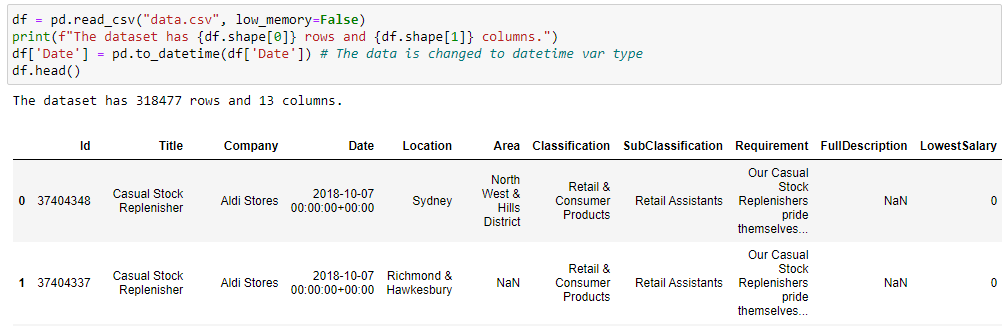
\includegraphics[scale = 0.56]{LoadingDataCode.png}
	\caption{Loading the Data with Pandas}
	\label{fig:LoadingData}
\end{figure}

As seen in figure \ref{fig:LoadingData}, the .csv file is read in and stored as a DataFrame type in the variable df. The head of the dataframe is then printed for visualisation purposes.\\
The first step to begin working with the data is to load it into a DataFrame using Pandas. Pandas is a flexible and powerful open-source data analytics tool, built for use in Python. To load the csv file into a DataFrame, just call read\_csv with the filename. In this assignment, an optional parameter "low\_memory=False" is also provided, to allow Pandas to use enough memory to determine the correct datatype for each column due to the size of the dataset. Without this parameter, Pandas will attempt to guess the datatypes, which may lead to unexpected results. To normalize the data, the average salary is calculated for all job entries, by taking the LowestSalaray and HighestSalary columns, and placed back into the DataFrame as a new column AverageSalary. This number is then multiplied by 1,000 and formatted for easier readabilitiy. This results in an average salary looking like "15,000" instead of "15.0". Normalizing the data this way provides each job entry with a fair visualisation of salary.

The dataset also requires some cleaning for a couple of the columns. The "Id" column is how Seek keeps track of unique job entries and should be an integer number, but occasionally contains some random characters. To clean this up, a regular expression is used to remove any occurence of characters that occur after - and including - an ampersand. The "Date" column also contains extra information that is not necessary for this analysis. This column includes hours, minutes, and seconds, but only the day, month, and year are required. To clean this column, a regular expression is used to remove anything after and including a 'T' character. This results in the "Date" column only containing the necessary information in the format yyyy-mm-dd. After the data cleaning is complete, the correct dtypes are assigned to the "Id" and "Date" columns.

\subsection{Hypothesis About the Analysis Outcome}

One expected outcome of the data analysis is the number of jobs based on location. The expected result is that jobs will be concentrated on the coast, with the highest number seen in the five large cities of Australia. A similar outcome is expected for the salaries of jobs; the further South you go - Melbourne, Sydney, Adelaide - the higher paying jobs you can expect to find. This is due to a large population density and higher cost of living in the Southern cities of Australia.

\newpage 
\section{Data Analysis and Interpretation}
%This section involves performing exploratory analysis, performing statistical analysis and performing predictive analysis on the job market dataset. 
\subsection{Studying the Job Meta Data / Attributes}

\begin{figure}[h]
	\centering
	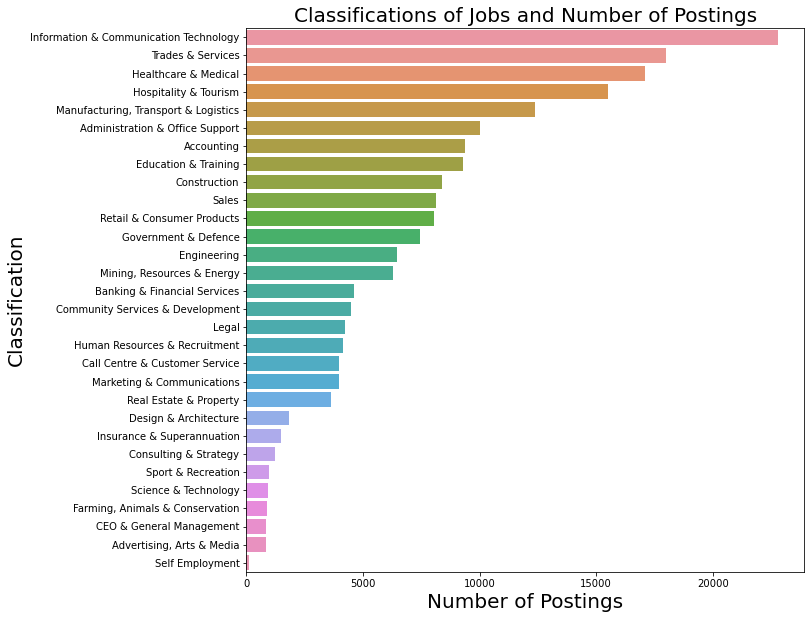
\includegraphics[scale = 0.45]{ClassVsPostings.png}
	\caption{Classification of Jobs and Number of Postings}
	\label{fig:ClassVsPosts}
\end{figure}

\begin{figure}[h!]
	\centering
	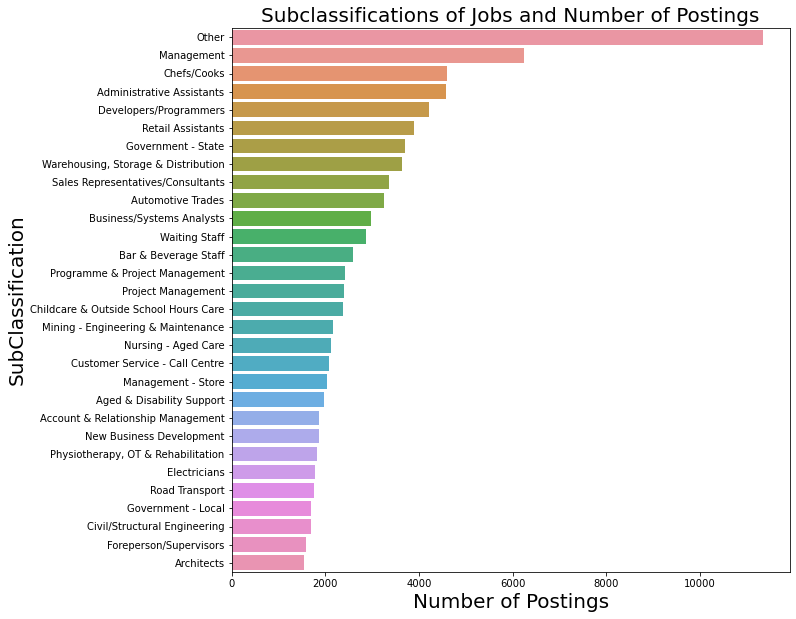
\includegraphics[scale = 0.45]{SubClassVsPostings.png}
	\caption{Subclassification of Jobs and Number of Postings}
	\label{fig:SubClassVsPosts}
\end{figure}

\newpage 
Figure \ref{fig:ClassVsPosts} shows the 30 unique job classifications from the market dataset. Figure \ref{fig:ClassVsPosts} also shows the posting frequency of each of these classifications with information and communication technology, trades and services, healthcare and medical, hospitality and tourism and manufacturing, transport and logistics being in the top five. Figure \ref{fig:SubClassVsPosts} shows the top 30 sub classifications from the market dataset. Figure \ref{fig:SubClassVsPosts} also shows the posting frequency of each of these sub classifications with other, management, chefs / cooks, administrative assistants and developers / programmers being in the top five. 

\begin{figure}[h!]
	\centering
	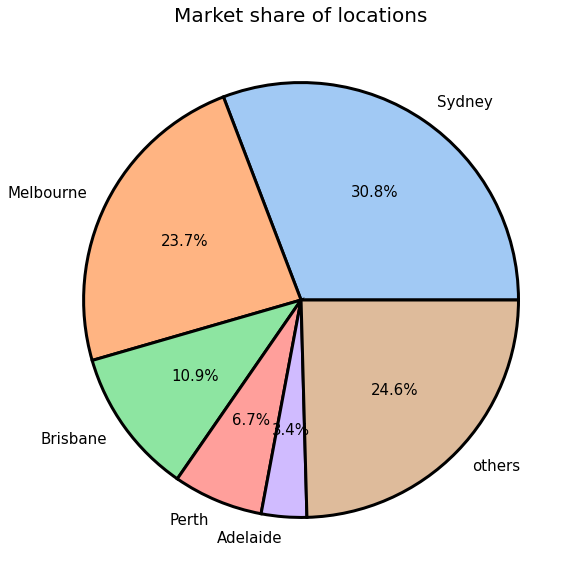
\includegraphics[scale = 0.60]{TopCities.png}
	\caption{Top Five Cities for Market Share}
	\label{fig:TopFiveCities}
\end{figure}

Figure \ref{fig:TopFiveCities} shows the top five cities in Australia in terms of market share from the dataset. It is clear that Sydney holds the highest market share of employment at 30.8\%, Melbourne in second with 23.7\% of the market share and Brisbane in third with 10.9\% of the market share. The other categories represents all other cities in Australia, and accounts for 24.6\% of the market. Adelaide presents the lowest market share at 3.4\% of the top five cities.\\
In the location analysis, the top three cities Sydney, Melbourne and Brisbane will be studied in terms of the market size in each city area, the hottest job sectors, the average salaries and the job posting dates for their respective job listings. 
\newpage
\begin{figure}[h]
	\centering
	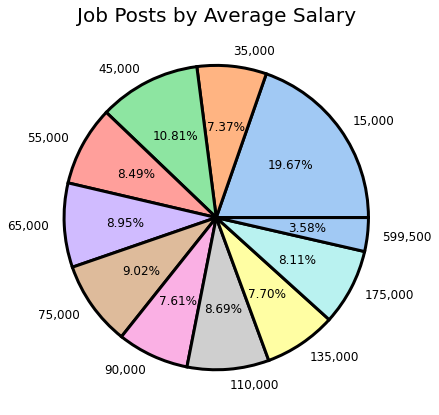
\includegraphics[scale = 0.55]{AverageRanges.png}
	\caption{Average Salary Ranges of Jobs}
	\label{fig:AverageRanges}
\end{figure}

Figure \ref{fig:AverageRanges} shows the average salary range distribution for all of the listed jobs. As seen in this chart, the most common salary is \$15,000 at 19.67\%. Jobs at this salary can expect around \$7.50 per hour working 40 hours a week, 50 weeks a year with 2 weeks of holidays. The highest average salary is around \$599,500 at 3.58\%. Jobs at this salary can expect around \$299.75 per hour working 40 hours a week, 50 weeks a year with 2 weeks of holidays. 

\begin{figure}[h]
	\centering
	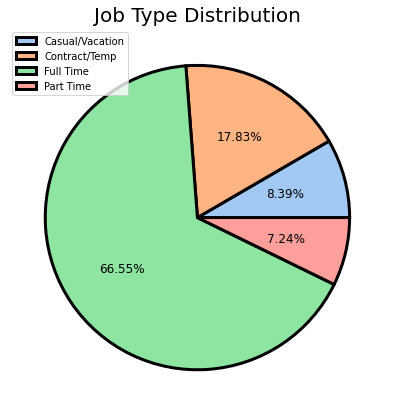
\includegraphics[scale = 0.55]{JobType.png}
	\caption{Distribution of Job Types}
	\label{fig:JobTypes}
\end{figure}

Figure \ref{fig:JobTypes} shows the distribution of advertised job types. From this pie chart it is clear that most jobs are under the job type "Full Time" at 66.55\%, whilst the smallest number of jobs fall under the job type "Part Time" at 7.24\%. 

\newpage
\subsection{Studying the Market by Locations}

\begin{figure}[h!]
	\centering
	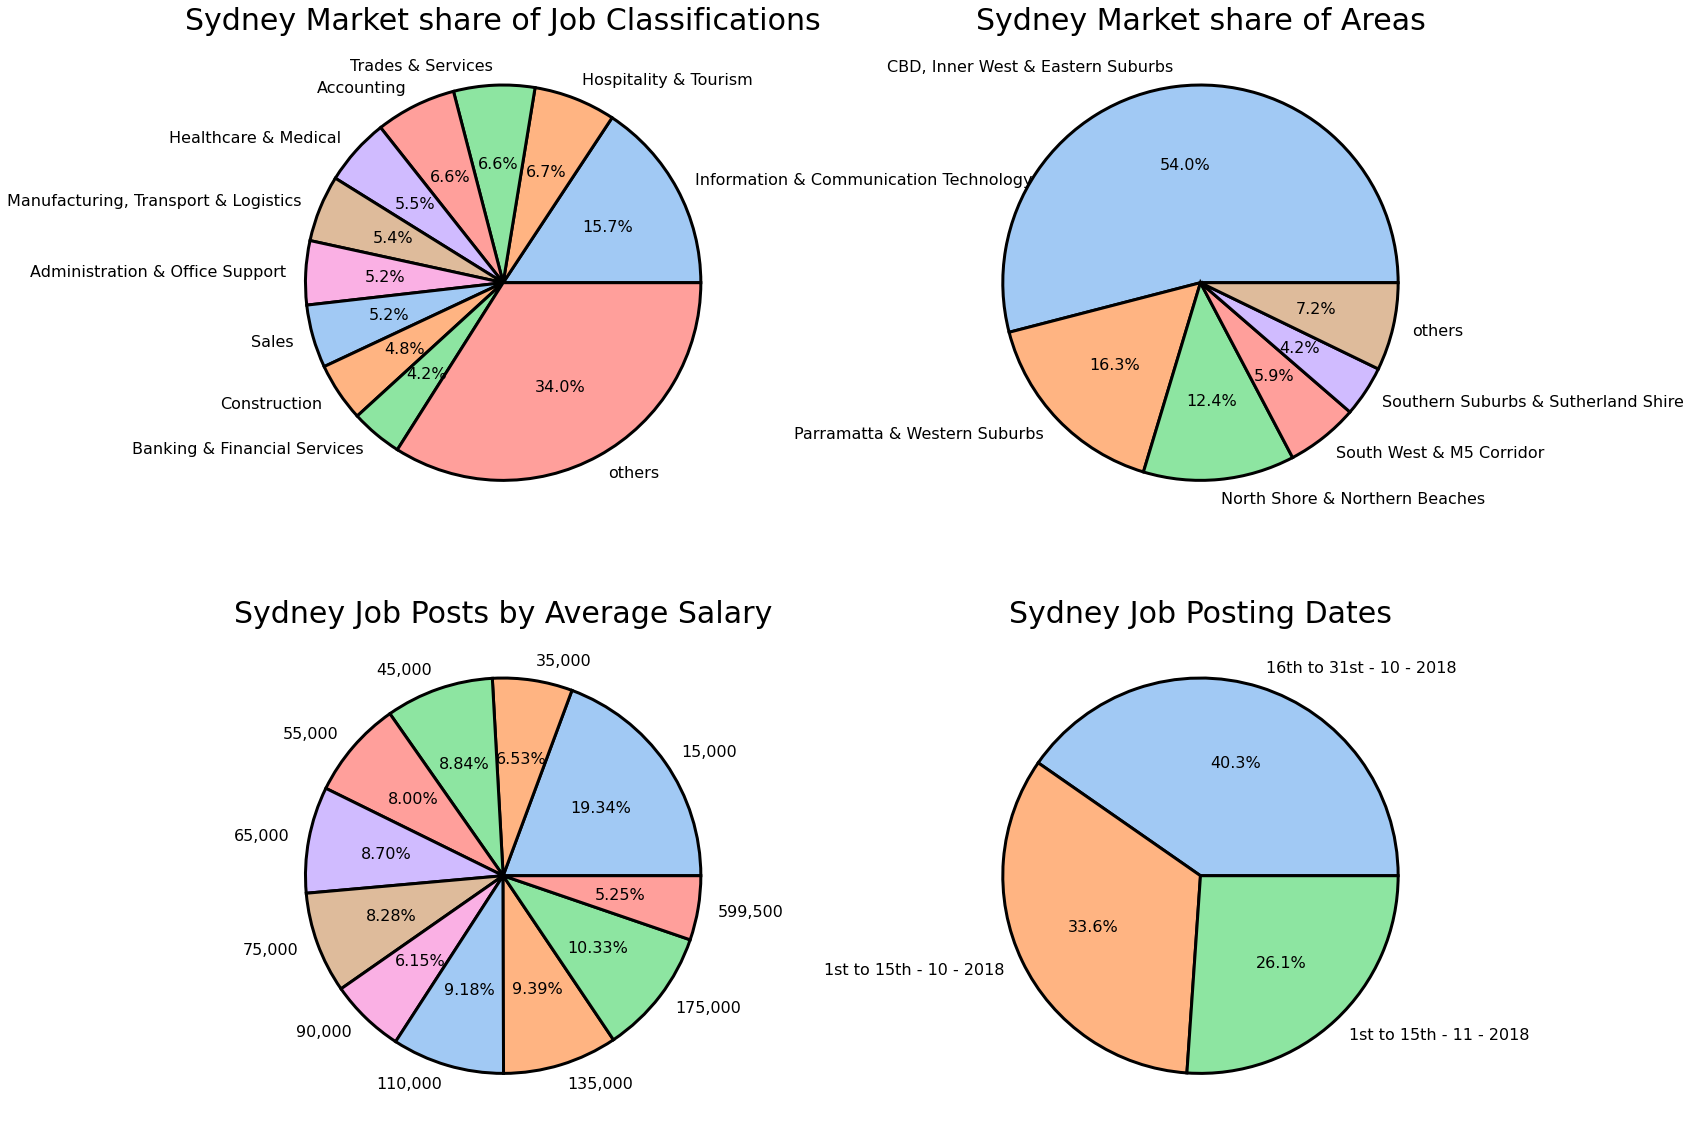
\includegraphics[scale = 0.26]{SydneyLocational.png}
	\caption{Sydney Locational Analysis}
	\label{fig:SydneyLoc}
\end{figure}

\begin{figure}[h!]
	\centering
	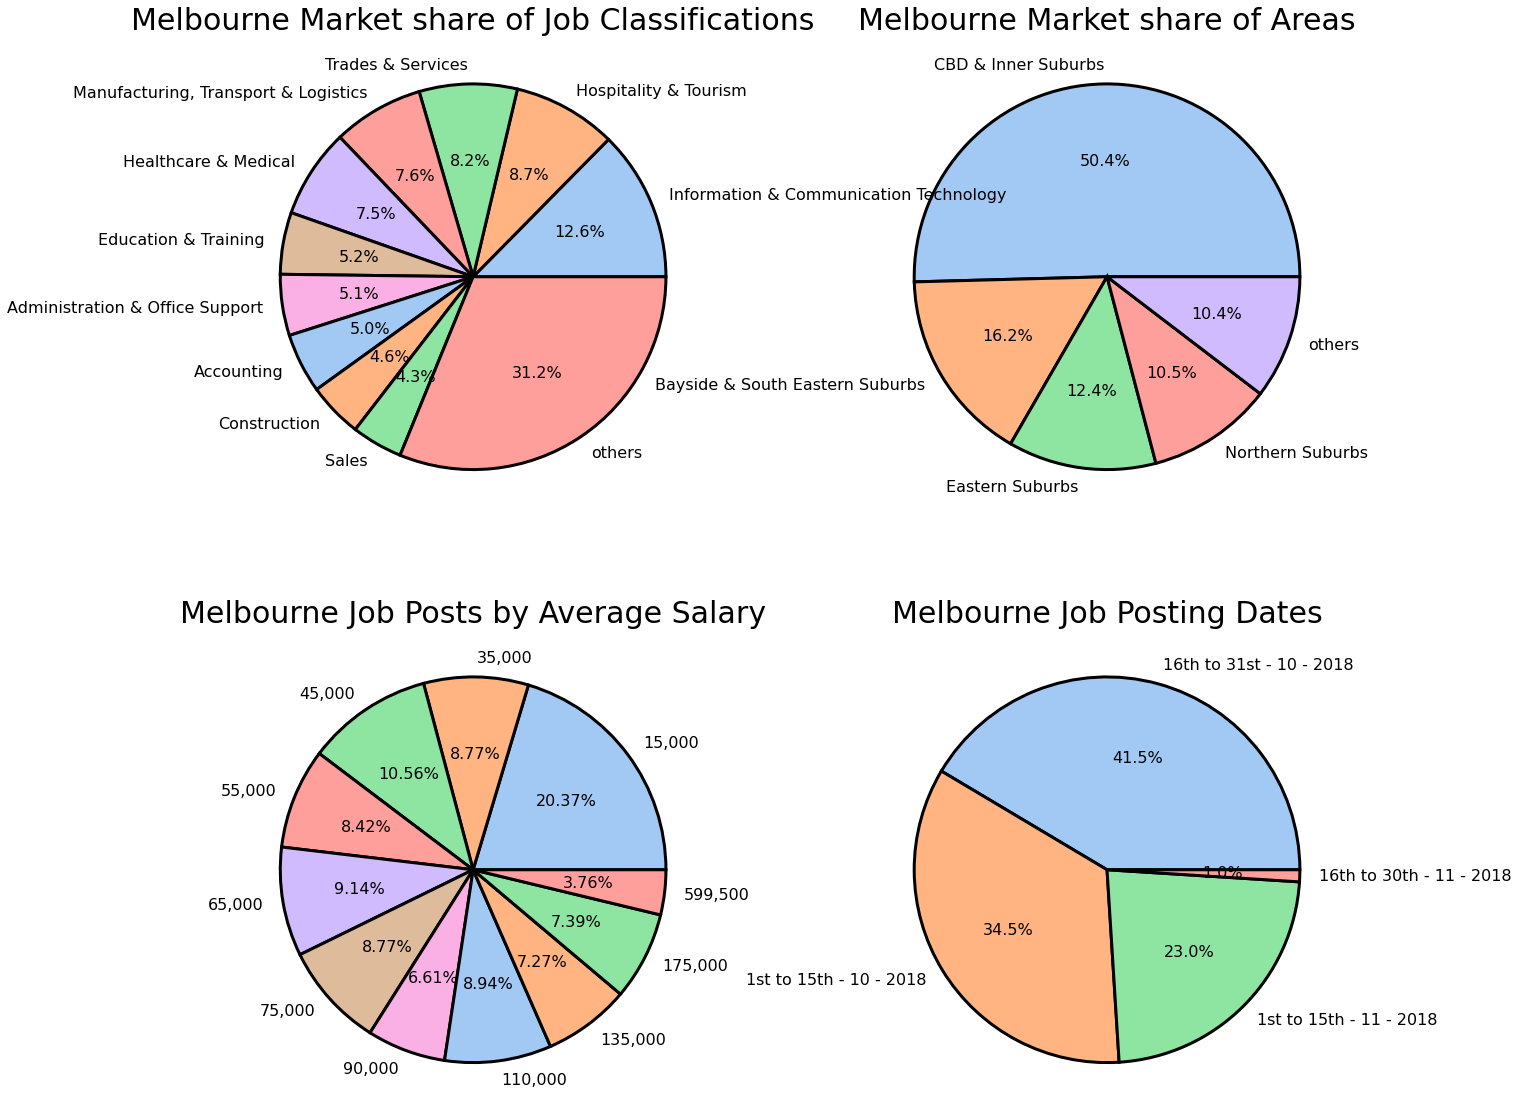
\includegraphics[scale = 0.26]{MelbourneLocational.png}
	\caption{Melbourne Locational Analysis}
	\label{fig:MelbLoc}
\end{figure}

\newpage
\begin{figure}[h]
	\centering
	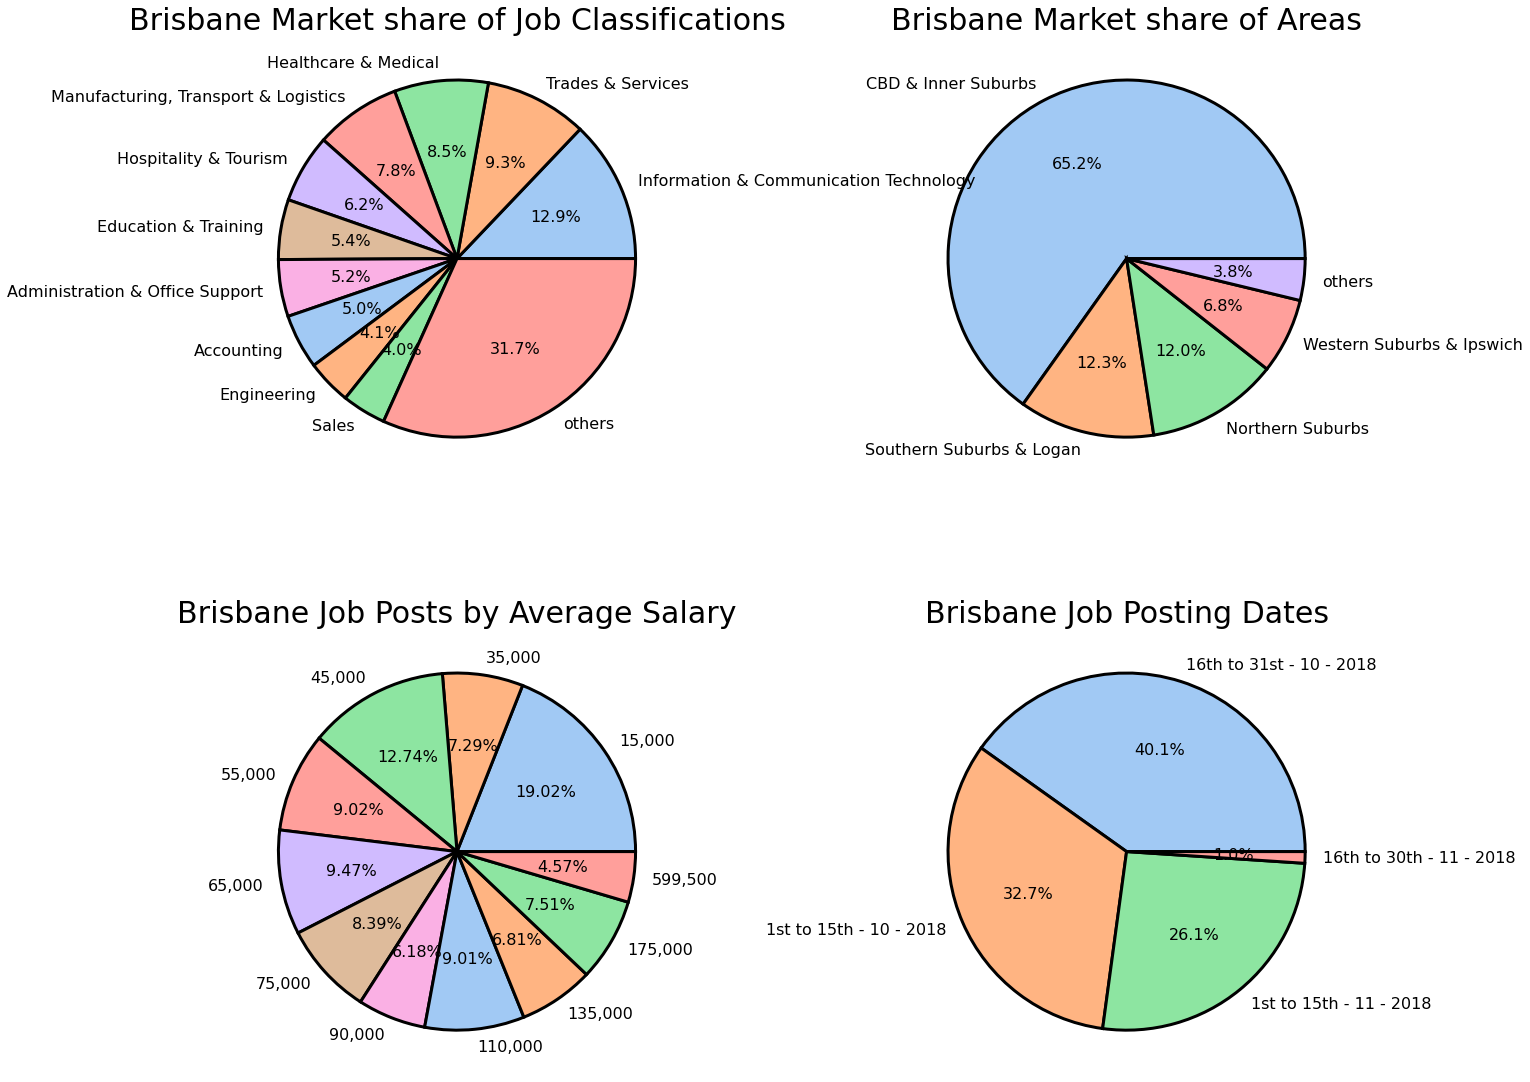
\includegraphics[scale = 0.26]{BrisbaneLocational.png}
	\caption{Brisbane Locational Analysis}
	\label{fig:BrisLoc}
\end{figure}

As seen in figure \ref{fig:SydneyLoc}, the Sydney job market is cornered by the information and communication technology sector which contributes to 15.7\% of the advertised jobs. More than half of the jobs, 54\%, of the market in Sydney are within the CBD, Inner West and Eastern Suburbs. The average salary for the advertised jobs in Sydney is \$15,000 taking up 19.34\%, of the advertised jobs. The least common average salary in Sydney is also the highest at \$599,500 taking up 5.25\% of advertised jobs. The majority of jobs, at 40.3\%, were listed in the second half of October, and 33.6\% and 26.1\% of the jobs were posted in the first half of October and November respectively. The least amount of jobs were advertised in the second half of November at 0\%.\\
As seen in figure \ref{fig:MelbLoc}, the Melbourne job market is also made up with a majority of listings in information and communication technology at 12.6\% of total job listings. The clear majority of job listings in Melbourne are in the CBD and Inner Suburbs of the city. The highest average salary from the job listings in Melbourne is \$15,000 which take up 20.37\% of the advertised jobs. The least common average salary is \$599,500 which consist of 3.76\% of the advertised jobs. Most of the jobs advertised in Melbourne were added in the second half of October at 41.5\% of listings and the first half of October at 34.5\%. The least amount of jobs were listed in the second half of November at 1\%.\\
As seen in figure \ref{fig:BrisLoc}, the highest advertised job in Brisbane is again, information and communication technology at 12.9\% of total job listings. The majority of the advertised jobs in Brisbane are located within the CBD and inner suburbs, accounting for 65.2\% of listings. The average salary in Brisbane is also \$15,000, at 19.02\% of listings, with \$599,500 once again being the least common listed salary at 4.57\% of total listings. Most of the jobs in Brisbane were listen in the second half of October at 40.1\% and the first half of October at 32.7\%. The least amount of jobs were listed in the second half of November at 1\%. 

\newpage
\subsection{Studying the Market by Sectors}

\begin{figure}[h]
	\centering
	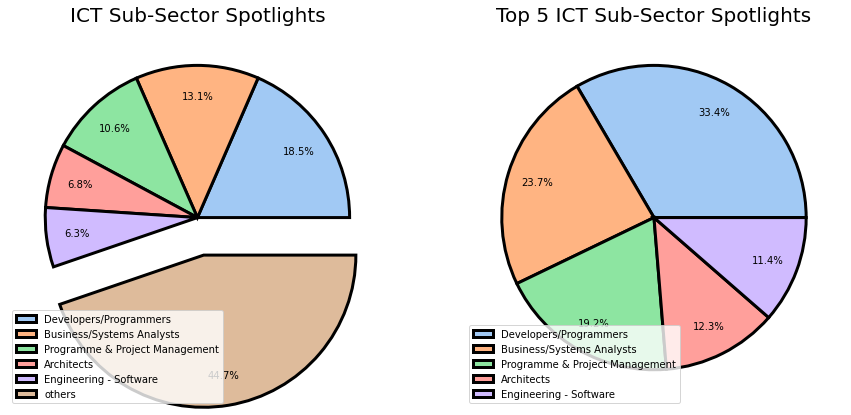
\includegraphics[scale = 0.50]{ICTspotlights.png}
	\caption{ICT Sub-Sector Spotlights}
	\label{fig:ICTspotlight}
\end{figure}

Figure \ref{fig:ICTspotlight} displays the top five sub-sector spotlights for the ICT job sector. As seen, developers/programmers is the highest listed sub-sector, accounting for 33.4\% of the job listings within ICT. A close second and third are business/systems analysis and programme \& project management, taking up 23.7\% and 19.2\% of the job listings in ICT respectively. 

\begin{figure}[h]
	\centering
	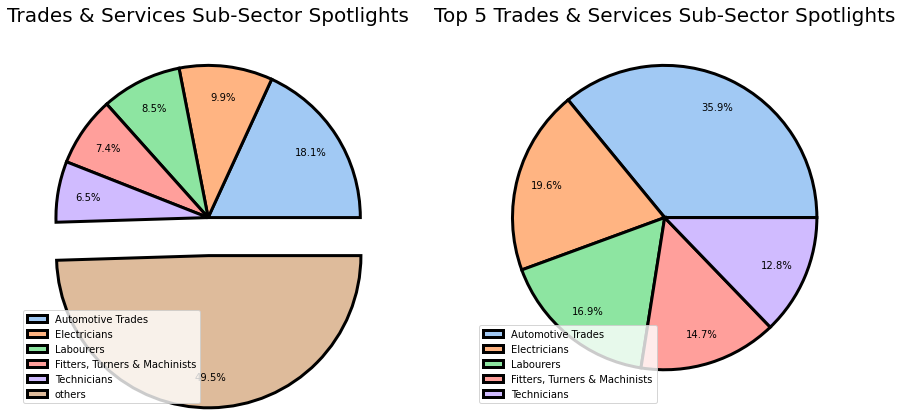
\includegraphics[scale = 0.50]{Tradespotlights.png}
	\caption{Trades and Services Sub-Sector Spotlights}
	\label{fig:Tradespotlight}
\end{figure}

Figure \ref{fig:Tradespotlight} displays the top five sub-sector spotlights for the trades and services job sector. As seen, automotive trades is the highest listed sub-sector, accounting for 35.9\% of the job listings within trades and services. Second and third are electricians and labourers, taking up 19.6\% and 16.9\% of the job listings in trades and services respectively. 

\newpage
\begin{figure}[h]
	\centering
	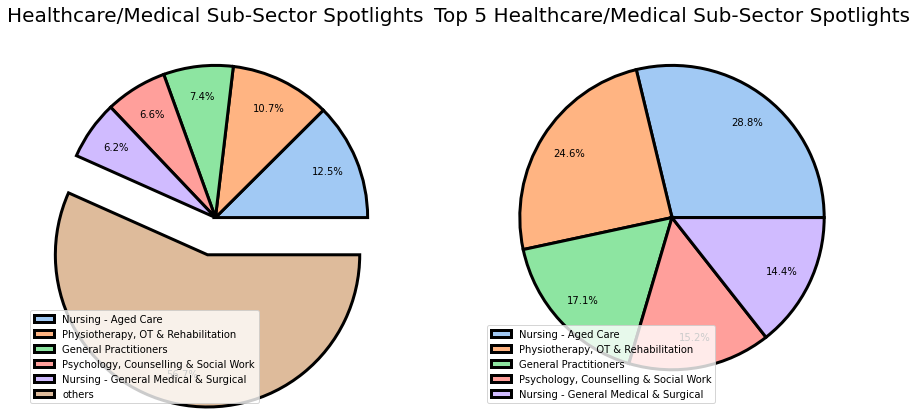
\includegraphics[scale = 0.50]{Healthspotlight.png}
	\caption{Healthcare and Medical Sub-Sector Spotlights}
	\label{fig:Healthspotlight}
\end{figure}

Figure \ref{fig:Healthspotlight} displays the top five sub-sector spotlights for the healthcare and medical job sector. As seen, nursing/aged care is the highest listed sub-sector, accounting for 28.8\% of the job listings within healthcare and medical. A close second and third are physiotherapy, OT \& rehabilitation and general practitioners, taking up 24.6\% and 17.1\% of the job listings in healthcare and medical respectively. 

\begin{figure}[h]
	\centering
	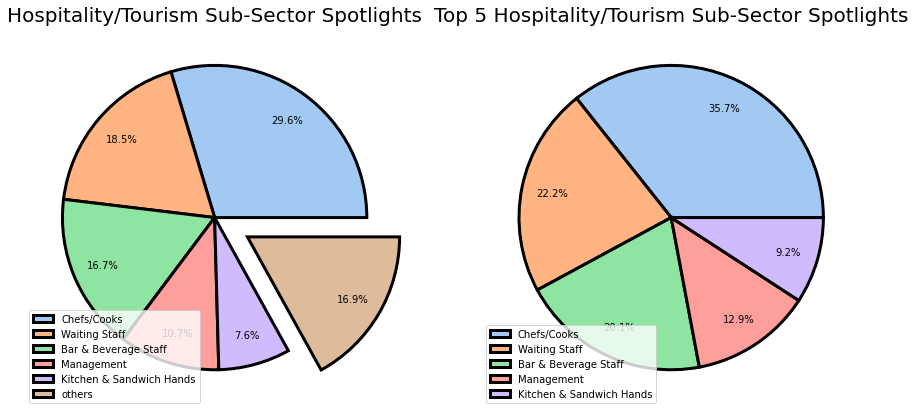
\includegraphics[scale = 0.50]{Hopsspotlight.png}
	\caption{Hospitality and Tourism Sub-sector Spotlights}
	\label{fig:Hospspotlight}
\end{figure}

Figure \ref{fig:Hospspotlight} displays the top five sub-sector spotlights for the hospitality and tourism job sector. As seen, chefs/cooks is the highest listed sub-sector, accounting for 35.7\% of the job listings within hospitality and tourism. A close second and third are waiting staff and bar \& beverage staff, taking up 22.2\% and 20.1\% of the job listings in hospitality and tourism respectively. 

\newpage
\begin{figure}[h]
	\centering
	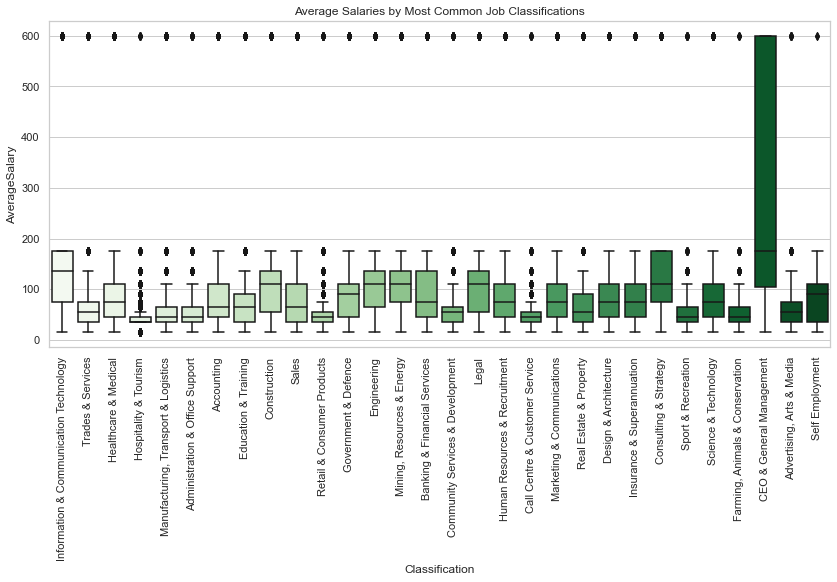
\includegraphics[scale = 0.50]{SectorAvgSalBox.png}
	\caption{Average Salary Range for Job Sectors}
	\label{fig:AvgSalBox}
\end{figure}

Figure \ref{fig:AvgSalBox} shows the breakdown of average salaries in each job classification, sorted from most common to least common jobs. As seen in the boxplot, ICT is the most common job and has the highest median salary, besides CEO \& General Management. Also present in the boxplot are the outliers in every classification. This is likely due to how some jobs may be listed as contract work and specify their rate in hourly or daily pay, which affects the data when pulled from the website.\\

As seen in figure \ref{fig:ClassVsPosts}, the highest sector of advertised jobs is the information \& communication systems sector. Information \& communication technology is the most listed job sector in the three biggest cities of Australia, Sydney, Melbourne and Brisbane, as evidenced in figures \ref{fig:SydneyLoc}, \ref{fig:MelbLoc} and \ref{fig:BrisLoc}, contributing to 15.7\%, 12.6\% and 12.9\% of the job listings respectively. In this job sector, the hottest sub-sectors are developers/programmers, business/systems analysts and programmers \& project management as seen in figure \ref{fig:ICTspotlight}, contributed to 33.4\%, 23.7\% and 19.2\% of the job listings respectively. The information \& communication systems sector is also one of the best paying sectors with a median average pay of around \$150,000 as seen in figure \ref{fig:AvgSalBox}. This is much higher than every other job sector except for CEO and general management. Therefore, since there is such a strong market trend in favour of ICT employability, it is recommended that a high school student considers a career in this sector to guarantee a job in the future. They should consider learning ICT relevant degrees in university such as IT, computer science or web development to acquire suitable skill sets to enter this job market. 

\newpage
\section{Evaluation}
\subsection{Findings of Data Analytics}
After conducting data analysis on the job meta data, locational analysis on the market and studying the market by sectors, there are clear trends in the job advertising in Australia. Looking at the market share of job listings in Australia, the top 5 cities were Sydney, Melbourne, Brisbane, Perth and Adelaide at 30.8\%, 23.7\%, 10.9\%, 6.7\% and 3.4\% respectively, as seen in figure \ref{fig:TopFiveCities}. The top five job posts by average salary were at \$15,000, \$45,000, \$75,000, \$65,000 and \$110,000 at 19.67\%, 10.81\%, 9.02\%, 8.95\% and 8.69\% respectively. For the sake of data analysis, all of these salaries were assumed to be yearly salaries. As seen in figure \ref{fig:JobTypes}, the clear majority of advertised jobs were for full time work at 66.55\%, followed by contract/temp work at 17.83\%. The least amount of advertised jobs were of the part time type at 7.24\%.\\
Locational data analysis was conducted for the top three cities in Australia, Sydney, Melbourne and Brisbane since they occupy a collective 65.4\% of the market share for job advertisements. It was seen in figure \ref{fig:SydneyLoc} that most of the jobs in Sydney were located in the CBD, inner west and eastern suburb areas at 54\%. As seen in figure \ref{fig:MelbLoc}, most of the jobs in Melbourne were also located in the CBD and inner suburbs at 50.4\%, while the same area for Brisbane occupies 65.2\% of job listings, as seen in figure \ref{fig:BrisLoc}.\\
In Sydney, the most advertised sector was information \& communication technology contributing 15.7\% of the job listings. This was followed by hospitality \& tourism, trades \& services and accounting at 6.7\%, 6.6\%, and 6.6\% respectively. In Melbourne, the most advertised sector was also information \& communication technology contributed to 12.6\% of the advertised job listings, followed by hospitality \& tourism, trades \& services and manufacturing, transport \& logistics at 8.7\%, 8.2\% and 7.6\% respectively. In Brisbane, information \& communication technology is again the most advertised sector at 12.9\%, followed by trades \& services, healthcare \& medical and manufacturing, transport \& logistics at 9.3\%, 8.5\% and 7.8\% respectively.\\
The average salary for job postings in Sydney were predominately at \$15,000 which contributed to 19.34\% of job listings, followed by \$175,000, \$135,000 and \$110,000 at 10.33\%, 9.39\% and 9.18\% respectively. The average job postings in Melbourne were also mostly at \$15,000, contributing to 20.37\% of advertised jobs, followed by \$175,000, \$135,000 and \$110,000 at 10.33\%, 9.39\% and 9.18\% respectively. The average job postings in Brisbane were mostly \$15,000, followed by \$45,000, \$65,000 and \$55,000 at 12.74\%, 9.47\% and 9.02\% respectively. In Sydney, Melbourne and Brisbane, the lowest advertised job had the highest salary at \$599,500, contributing to 5.52\%, 3.76\% and 4.57\% of advertised jobs respectively in each city. It is clear that the job market in Sydney and Melbourne pays much higher than the jobs in Brisbane on average.\\ 
40.3\% of jobs in Sydney were posted in the first half of October 2018, whilst 33.6\% and 26\% of the jobs were posted in the first halves of October and November respectively. 41.5\% of jobs in Melbourne were posted in the second half of October, with 34.5\% and 23\% of jobs posted in the second halves of October and November respectively. 40.1\% of jobs in Brisbane were posted in the second half of October, with 32.7\% and 26.1\% of jobs advertised in the second halves of October and November respectively. There is a clear trend in the job advertisement dates for these three cities as they have very similar distributions of postings. This means that there is a surge in advertisement for jobs towards the end of the year, but drop off dramatically in the second half of October.\\
After sectional analysis on the job markets, it is more clear which sectors are more frequency advertised. Sub-sector analysis was conducted for the top four sectors, information \& communication technology, trades \& services, healthcare/medical and hospitality/tourism. As seen in figure \ref{fig:ICTspotlight}, the top five sub-sectors in the information \& communication technology sector are developers/programmers, business/systems analysts, programmer/project management, architects and engineering - software, at 33.4\%, 23.7\%, 19.2\%, 12.3\% and 11.4\% of the top five sub-sectors respectively. As seen in figure \ref{fig:Tradespotlight}, the top five sub-sectors in the trades \& services sector are automotive trades, electricians, labourers, fitters turners \& machinists and technicians, at 35.9\%, 19.6\%, 16.9\%, 14.7\% and 12.8\% of the top five sub-sectors respectively. As seen in figure \ref{fig:Healthspotlight}, the top five sub-sectors in the healthcare/medical sector are nursing - aged care, physiotherapy OT \& rehabilitation, general practitioners, psychology counselling \& social work and nursing general medical \& surgical, at 28.8\%, 24.6\%, 17.1\%, 15.2\% and 14.4\% of the top five sub-sectors respectively. As seen in figure \ref{fig:Hospspotlight}, the top five sub-sectors in the hospitality/tourism sector are chefs/cooks, waiting staff, bar \& beverage staff, management and kitchen \& sandwich hands, at 35.7\%, 22.2\%, 20.1\%, 12.9\% and 9.2\% of the top five sub-sectors respectively. After this analysis, the top sub-sectors of the top four sectors are developers/programmers, automotive trades, nursing-aged care and chefs/cooks.\\
Figure \ref{fig:AvgSalBox} shows a box plot for average salaries of each advertised job sector. It is clear that the job with the highest variance is the CEO \& general management sector. These jobs start at just over \$100,000 and reach up to around \$600,000. Compared with the sector analysis, the information \& communication technology sector is well paid starting at around \$80,000 and reaching around \$180,000. The median of this sector is around \$150,000, which is the highest median other than the CEO \& general management sector.The second most advertised sector, trades \& services is a relatively low paying field with its highest paying positions reaching the median of an ICT job. The third most advertised sector, healthcare/medical has a lower median average pay than ICT jobs, but has similar top paying jobs. The fourth most advertised sector of hospitality/tourism has significantly lower paid job opportunities, but with high paid outliers. These outliers are most likely due to contract or short term work however and are not necessarily indicative of a yearly salary.\\
The data analysis has indicated that the ICT sector is a clear best choice for a future job since it is the most advertised sector in the biggest three cities in Australia, and has the second highest median average pay. 

\subsection{Balancing the Market}

\newpage
\subsection{Refining the Data Analytics}




\subsection{Implications for Employers and Employees}

\newpage
\section{Case Studies}
\subsection{Case Study 1}
\subsection{Case Study 2}



\end{document}
